\documentclass[a4paper]{article}
%\usepackage{vntex}
%\usepackage[english,vietnam]{babel}
%\usepackage[utf8]{inputenc}

%\usepackage[utf8]{inputenc}
%\usepackage[francais]{babel}
\usepackage{a4wide,amssymb,epsfig,latexsym,multicol,array,hhline,fancyhdr}

\usepackage{amsmath}
\usepackage[framemethod=tikz]{mdframed}
\usepackage{lastpage}
\usepackage[lined,boxed,commentsnumbered]{algorithm2e}
\usepackage{enumerate}
\usepackage{alltt}
\usepackage{color}
\usepackage{xcolor}
\usepackage{graphicx}							% Standard graphics package
\usepackage{array}
\usepackage{tabularx, caption}
\usepackage{multirow}
\usepackage{multicol}
\usepackage{rotating}
\usepackage{booktabs}
\usepackage{graphics}
\usepackage{geometry}
\usepackage{setspace}
\usepackage{amsmath}
\usepackage{epsfig}
\usepackage{tikz}
\usetikzlibrary{arrows,snakes,backgrounds}
\usepackage{hyperref}
\hypersetup{urlcolor=blue,linkcolor=black,citecolor=black,colorlinks=true} 
%\usepackage{pstcol} 								% PSTricks with the standard color package

%\newtheorem{theorem}{{\bf Định lý}}
%\newtheorem{property}{{\bf Tính chất}}
%\newtheorem{proposition}{{\bf Mệnh đề}}
%\newtheorem{corollary}[proposition]{{\bf Hệ quả}}
%\newtheorem{lemma}[proposition]{{\bf Bổ đề}}

\DeclareMathOperator*{\argmax}{argmax}
%\usepackage{fancyhdr}
\setlength{\headheight}{40pt}
\pagestyle{fancy}
\fancyhead{} % clear all header fields
\fancyhead[L]{
 \begin{tabular}{rl}
    \begin{picture}(25,15)(0,0)
    \put(0,-8){
\includegraphics[width=8mm, height=8mm]{hcmut.png}}
    %\put(0,-8){\epsfig{width=10mm,figure=hcmut.eps}}
   \end{picture}&
	%
\includegraphics[width=8mm, height=8mm]{hcmut.png} & %
	\begin{tabular}{l}
		\textbf{\bf \ttfamily Ho Chi Minh University of Technology}\\
		\textbf{\bf \ttfamily Faculty of Computer Science and Engineering}
	\end{tabular} 	
 \end{tabular}
}
\fancyhead[R]{
	\begin{tabular}{l}
		\tiny \bf \\
		\tiny \bf 
	\end{tabular}  }
\fancyfoot{} % clear all footer fields
\fancyfoot[L]{\scriptsize \ttfamily Assignment 1 - System call}
\fancyfoot[R]{\scriptsize \ttfamily Page {\thepage}/\pageref{LastPage}}
\renewcommand{\headrulewidth}{0.3pt}
\renewcommand{\footrulewidth}{0.3pt}


%%%
\setcounter{secnumdepth}{4}
\setcounter{tocdepth}{3}
\makeatletter
\newcounter {subsubsubsection}[subsubsection]
\renewcommand\thesubsubsubsection{\thesubsubsection .\@alph\c@subsubsubsection}
\newcommand\subsubsubsection{\@startsection{subsubsubsection}{4}{\z@}%
                                     {-3.25ex\@plus -1ex \@minus -.2ex}%
                                     {1.5ex \@plus .2ex}%
                                     {\normalfont\normalsize\bfseries}}
\newcommand*\l@subsubsubsection{\@dottedtocline{3}{10.0em}{4.1em}}
\newcommand*{\subsubsubsectionmark}[1]{}
\makeatother


\begin{document}

\begin{titlepage}
\begin{center}
\Large{HO CHI MINH CITY UNIVERSITY OF TECHNOLOGY \\
FACULTY OF COMPUTER SCIENCE AND ENGINNERING}
\end{center}

\vspace{1cm}

\begin{figure}[h!]
\begin{center}

\includegraphics[width=3cm]{hcmut.png}
\end{center}
\end{figure}

\vspace{1cm}


\begin{center}
\begin{tabular}{c}
\multicolumn{1}{l}{\textbf{{\Large OPERATING SYSTEM (CO2017)}}}\\
~~\\
\hline
\\
\multicolumn{1}{l}{\textbf{{\Large Assignment 1 - Report}}}\\
\\
\textbf{{\Huge SYSTEM CALL}}\\
\\
\hline
\end{tabular}
\end{center}

\vspace{3cm}

\begin{table}[h]
\begin{tabular}{rrl}
\hspace{5 cm} & Lecturer: & Pham Trung Kien\\
& Student: & Doan Tran Huu Phuoc - 1813636 \\
\end{tabular}
\end{table}

\begin{center}
{\footnotesize Ho Chi Minh City, 05/2020}
\end{center}
\end{titlepage}


%\thispagestyle{empty}

\newpage
\tableofcontents
\newpage
%%%%%%%%%%%%%%%%%%%%%%%%%%%%%%%%%
\section{Introduction:}
\subsection{System calls:} 
System calls provide an interface to the services made available by an operating system. These calls are generally available as routines written in C and C++, although certain low-level tasks (for example, tasks where hardware must be accessed directly) may have to be written using assembly-language instructions.\\
As you can see, even simple programs may make heavy use of the operating system. Frequently, systems execute thousands of system calls per second. Most programmers never see this level of detail, however. Typically, application developers design programs according to an application programming interface (API). The API specifies a set of functions that are available to an application programmer, including the parameters that are passed to each function and the return values the programmer can expect. The functions that make up an API typically invoke the actual system calls on behalf of the application programmer.
\begin{figure}[h!]
\begin{center}
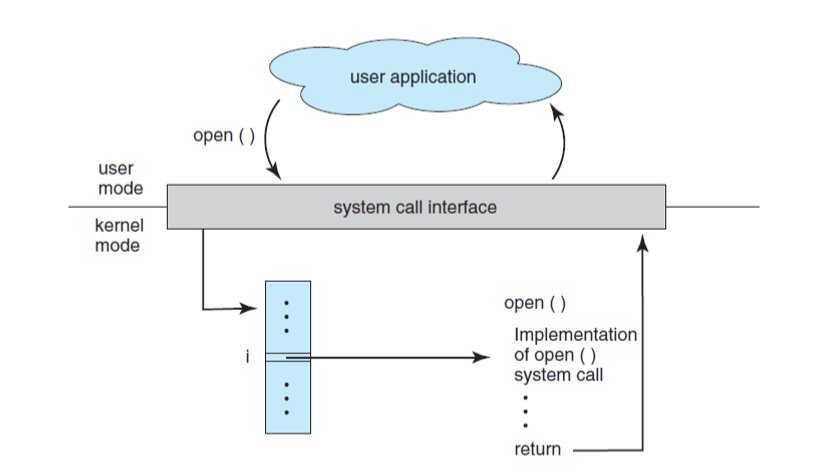
\includegraphics[width=14cm]{Intro.png}
\caption{The handling of a user application invoking the open() system call}
\end{center}
\end{figure}
\subsection{Goal of assignment:}
This assignment guides students compile a new Linux kernel. It requires that students implement a new system call getting some information of a process and add the new system call to the kernel.
\newpage
%%%%%%%%%%%%%%%%%%%%%%%%%%%%%%%%%
\section{Compiling Linux Kernel:}
\subsection{Preparation:}
\textbf{Set up Virtual Machine:} Download and install Ubuntu 18.04 on VMWare WorkStation 15 Player.\\
\textbf{Install the core packages:} Get Ubuntu's toolchain (gcc, make, and so forth) by installing the buildessential metapackage:\\
\noindent\fbox{%
\parbox{\textwidth}{%
\$ \texttt{sudo apt-get update} \\
\$ \texttt{sudo apt-get install build-essential}
}%
}\\
\\
Install kernel-package:\\
\noindent\fbox{%
\parbox{\textwidth}{%
\$ \texttt{sudo apt-get install kernel-package}
}%
}\\
\begin{mdframed}[hidealllines=true,backgroundcolor=blue!10]
\textbf{QUESTION:} Why we need to install kernel-package?
\begin{itemize}
\item[$\rightarrow$] \textbf{Answer:} There are a lot of advantages when installing kernel-package. If we compile kernel manually, there are many steps by steps that we need to follow strictly. Kernel-package include almost everything we need. Therefore, time spending on installing kernel will cut down a lot because it just need some commands to set up kernel with kernel-package. Besides, it allow us to:\\
 - Keep multiple versions of kernel-image on device without disturbing, make sure that installation files along with kernel-image of its always goes together.\\
 - Facilitate keeping multiple versions of the same kernel on device.\\
 - Automatically move folders to the appropriate location and select settings suitable for each architecture.\\
 - Kernel-models are linked, so it can be easily compiled and guaranteed compatible.\\
 - System can manage installed kernel versions.\\
 - Create packages with header files, source files as well as .deb files that are managed by the system manager (by Package Management System).\\
 - Compile kernel on many child architectures.\\
 - Compile kernel on other computers.
\end{itemize}
\end{mdframed}
\textbf{Create a kernel compilation directory:}\\
\noindent\fbox{%
\parbox{\textwidth}{%
\$ \texttt{mkdir ˜/kernelbuild}
}%
}\\
\\
\textbf{Download the kernel source:}\\
\noindent\fbox{%
\parbox{\textwidth}{%
\$ \texttt{cd ˜/kernelbuild}\\
\$ \texttt{ wget https:\textit{\color{blue}//cdn.kernel.org/pub/linux/kernel/v5.x/linux-5.0.5.tar.xz}}
}%
}\\
\newpage
\begin{mdframed}[hidealllines=true,backgroundcolor=blue!10]
\textbf{QUESTION:} Why we have to use another kernel source from the server such as\\
http://www.kernel.org, can we compile the original kernel (the local kernel on the running OS) directly?
\begin{itemize}
\item[$\rightarrow$] \textbf{Answer:} When using a kernel source, it is easy to edit, review directories and set up necessary patch.\\
It is unable to compile a kernel directly from itself. Meanwhile, it is possible to compile a kernel version similar to the current version, the source code can be obtained by the following command:\\
\texttt{apt-get source linux-image-\$(uname -r)}
\end{itemize}
\end{mdframed}
\textbf{Unpack the kernel source} as tarball format in the build directory: \\
\noindent\fbox{%
\parbox{\textwidth}{%
\$ \texttt{tar -xvJf linux-5.0.5.tar.xz}
}%
}\\
\subsection{Configuration:}
Copy the content of configuration file of the existing kernel currently used by the virtual machine to the source code directory. Then, we must install some essential packages to edit configure file through terminal interface.\\
\noindent\fbox{%
\parbox{\textwidth}{%
\$ \texttt{ cp /boot/config-\$(uname -r) ˜/kernelbuild/.config}
}%
}\\
\\
To edit configure file through terminal interface, we must install some essential packages:\\
\noindent\fbox{%
\parbox{\textwidth}{%
\$ \texttt{sudo apt-get install fakeroot ncurses-dev xz-utils bc flex libelf-dev bison}
}%
}\\
\\
Then, run \$ make menuconfig or \$ make nconfig to open Kernel Configuration.\\
\noindent\fbox{%
\parbox{\textwidth}{%
\$ \texttt{cd linux-5.0.5}\\
\$ \texttt{make nconfig}
}%
}\\
\\
\begin{figure}[h!]
\begin{center}
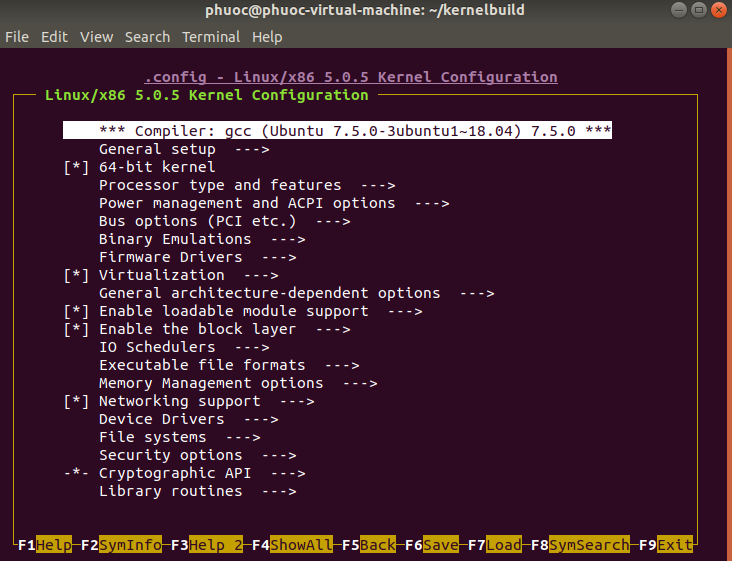
\includegraphics[width=8.5cm]{1.png}
\caption{Menu Kernel Configuration}
\end{center}
\end{figure}
Go to General setup option. Then access to the line \textbf{``(-ARCH) Local version - append to kernel release}. Then enter ``.1813636''.  Then press F6 to save the changes and press F9 to exit.\\
\begin{figure}[h!]
\begin{center}
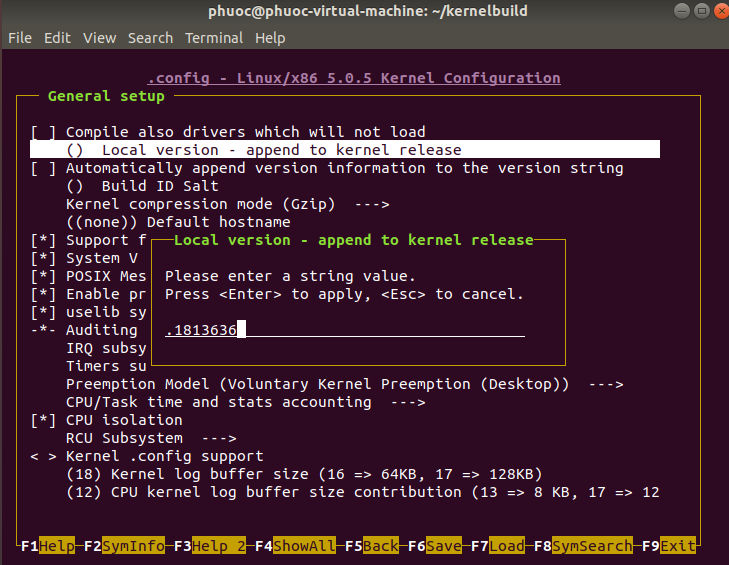
\includegraphics[width=8.5cm]{2.png}
\caption{Append student ID}
\end{center}
\end{figure}
\\
Install openssl package to encounter some errors. \\
\noindent\fbox{%
\parbox{\textwidth}{%
\$ \texttt{sudo apt-get install openssl linssl-dev}
}%
}\\
\\
\subsection{Build the configured kernel:}
Run \texttt{make -j 4} to compile the kernel and create the kernel ``vmlinuz''. Then build the loadable kernel modules by the command \texttt{make -j 4}.\\
\begin{mdframed}[hidealllines=true,backgroundcolor=blue!10]
\textbf{QUESTION:} What is the meaning of these two stages, namely “make” and “make modules”? What are created and what for?
\begin{itemize}
\item[$\rightarrow$] \textbf{Answer:} \texttt{make} creates a compressed version of kernel-image, used by \texttt{boot loader}. The command \texttt{make} connect the libraries to the source then create linkage between necessary files, set it up for the final stage and create binary files.\\
\texttt{make} modules compiles modules and leaves compiled binary files in the build directory
\end{itemize}
\end{mdframed}
\subsection{Installing the new kernel:}
First install the modules:\\
Install openssl package to encounter some errors. \\
\noindent\fbox{%
\parbox{\textwidth}{%
\$ \texttt{sudo make -j 4 modules\_install}
}%
}\\
\\
Then install the kernel itself:\\
\noindent\fbox{%
\parbox{\textwidth}{%
\$ \texttt{sudo make -j 4 install}
}%
}\\
\\
\textbf{Check out:} After installing the new kernel by steps described above, reboot the virtual machine by typing\\
Then install the kernel itself:\\
\noindent\fbox{%
\parbox{\textwidth}{%
\$ \texttt{sudo reboot}
}%
}\\
\\
After logging into the computer again, run the command \texttt{uname -r}. The output string contains the MSSV means your custom kernel has been compiled and installed successfully.
\begin{figure}[h!]
\begin{center}
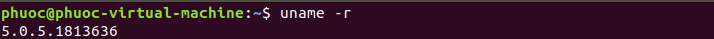
\includegraphics[width=14cm]{3.png}
\caption{Print out MSSV}
\end{center}
\end{figure}
%%%%%%%%%%%%%%%%%%%%%%%%%%%%%%%%%
\section{Trim the kernel:}
Display GRUB and comment out GRUB\_HIDDEN\_TIMEOUT\\
\noindent\fbox{%
\parbox{\textwidth}{%
\$ \texttt{sudo vim/etc/default/grub}\\
\$ \texttt{sudo update-grub}
}%
}\\
\\
Then trim the kernel by the following command:\\
\noindent\fbox{%
\parbox{\textwidth}{%
\$ \texttt{make localmodconfig}
}%
}\\
\\
\begin{figure}[h!]
\begin{center}
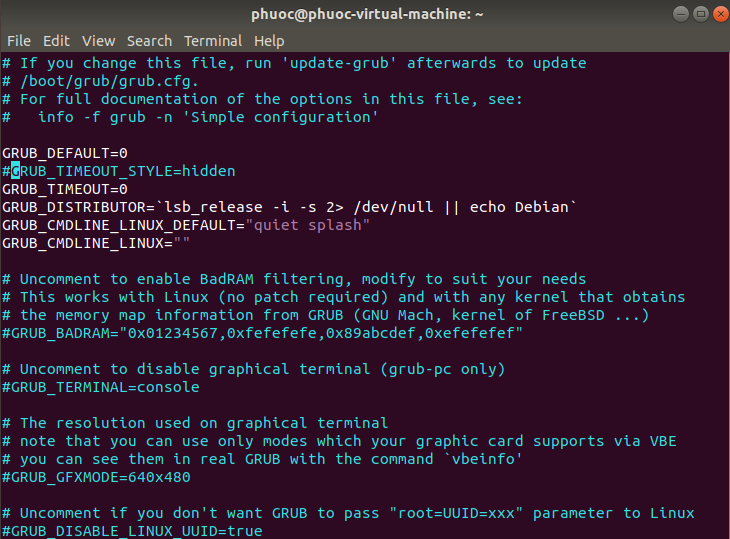
\includegraphics[width=8.5cm]{4.png}
\caption{Trim the kernel}
\end{center}
\end{figure}
\newpage
%%%%%%%%%%%%%%%%%%%%%%%%%%%%%%%%%
\section{System call:}
\subsection{Adding new system call:}
Create folder to store header files and source code files named get\_proc\_info.\\
\noindent\fbox{%
\parbox{\textwidth}{%
\$ \texttt{mkdir get\_proc\_info}\\
\$ \texttt{cd get\_proc\_info}
}%
}\\
\\
Then, we create a Makefile for the new system call function.\\
\noindent\fbox{%
\parbox{\textwidth}{%
\$ \texttt{vim Makefile}
}%
}\\
\begin{figure}[h!]
\begin{center}
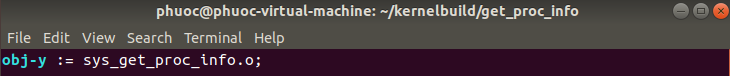
\includegraphics[width=14cm]{5.png}
\caption{Makefile of system call}
\end{center}
\end{figure}
\\
Create a Makefile for the source file\\
\noindent\fbox{%
\parbox{\textwidth}{%
\$ \texttt{cd ..}\\
\$ \texttt{vim Makefile}
}%
}\\
\begin{figure}[h!]
\begin{center}
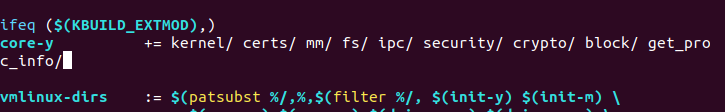
\includegraphics[width=14cm]{6.png}
\caption{Makefile of kernel}
\end{center}
\end{figure}
\\
Add the new system call to the system call table\\
\noindent\fbox{%
\parbox{\textwidth}{%
\$ \texttt{cd arch/x86/entry/syscalls/}\\
\$ \texttt{gedit syscall\_64.tbl}
}%
}\\
\begin{figure}[h!]
\begin{center}
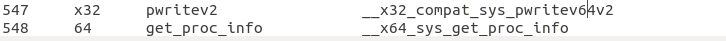
\includegraphics[width=14cm]{7.png}
\caption{Add system call to system call table}
\end{center}
\end{figure}
\begin{mdframed}[hidealllines=true,backgroundcolor=blue!10]
\textbf{QUESTION:} What is the meaning of fields of the line that just add to the system call table (548, 64, get\_proc\_info, i.e.)? 
\begin{itemize}
\item[$\rightarrow$] \textbf{Answer:} 
\begin{itemize}
\item[\textbullet] 548: the number of the entry of the new system call.
\item[\textbullet] 64: system call has a common implementation for both of the ABIs for x86 and 64 bit instruction.
\item[\textbullet] get\_proc\_info: using to declare as user.
\item[\textbullet] \_\_x64\_sys\_get\_proc\_info: name of function of the new system call inside kernel.
\end{itemize} 
\end{itemize}
\end{mdframed}
Add new system call to the system call header file:\\
\noindent\fbox{%
\parbox{\textwidth}{%
\$ \texttt{cd}\\
\$ \texttt{cd kernelbuild/include/linux/}\\
\$ \texttt{gedit syscalls.h}
}%
}\\
\begin{figure}[h!]
\begin{center}
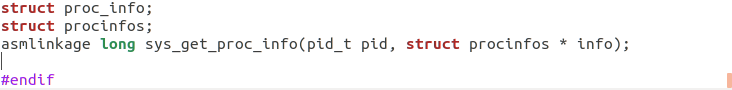
\includegraphics[width=14cm]{8.png}
\caption{Edit header file}
\end{center}
\end{figure}
\begin{mdframed}[hidealllines=true,backgroundcolor=blue!10]
\textbf{QUESTION:} What is the meaning of each line above? 
\begin{itemize}
\item[$\rightarrow$] \textbf{Answer:}
\begin{itemize}
\item[\textbullet]\texttt{\textbf{struct proc\_info}} and \texttt{struct proinfos}:\\
declare the structure used by the new system call.
\item[\textbullet]\texttt{\textbf{asmlinkage long sys\_get\_proc\_info(pid\_t pid, struct procinfos * info)}}:\\
specify the type of input parameters and the system call data type. \texttt{asmlinkage} make announcement that the function only accept parameters passed from register.
\end{itemize}
\end{itemize}
\end{mdframed}

\subsection{System call implementation:}
The new system call intents to extract information of a running process by its pid. We propose structures proc\_info and procinfos implemented in sys\_get\_proc\_info.c to keep information of process. We also need to get information of a process that is required by the input of its pid through sys\_get\_proc\_info function. Each process has its own task\_struct which help to get process’s name, pid, parent process, children process. To get the information of the process has given pid, we use the marco for\_each\_process(struct task\_struct defined in linux/sched.h). When this marco is running, it will check every single running process and store the information of process to passed parameters temporarily. As a result, we can get the information of the process and store it to procinfos structure. The specifical implementation was done in sys\_get\_proc\_info.c. Finally, the program ``testing.c'' was made to check the result.\\
\begin{figure}[h!]
\begin{center}

\includegraphics[width=14cm]{9.png}
\caption{Testing}
\end{center}
\end{figure}
\newpage
\begin{mdframed}[hidealllines=true,backgroundcolor=blue!10]
\textbf{QUESTION:} Why this program could indicate whether our system call works or not? 
\begin{itemize}
\item[$\rightarrow$] \textbf{Answer:}
It depends on the return value of the function\\
\texttt{sys\_return\_value = syscall([syscall\_number\_in\_tbl], pid, info)} to know if the new system call works or not. The value of he function returns 0 if success, otherwise, it returns EINVAL.
\end{itemize}
\end{mdframed}

\subsection{Compilation and Installation process:}
After setting things up, we proceed to compile and install kernel with the following commands:
\noindent\fbox{%
\parbox{\textwidth}{%
\$ \texttt{make -j 8}\\
\$ \texttt{make -j 8 modules}\\
\$ \texttt{sudo make -j 8 modules\_install}\\
\$ \texttt{sudo make -j 8 install}
}%
}\\
\\
Then reboot the system.
\subsection{Making API for system call:}
Although get proc info system call works properly, we still have to invoke it through its number which is quite inconvenient for other programmers so we need to implement a C wrapper for it to make it easy to use. This can be done outside the kernel. Thus, to avoid recompile the kernel again, we leave out kernel source code directory and create another directory to store source code for our wrapper. We first create a header file which contains the prototype of the wrapper and declare procinfos and proc info struct. \\
\noindent\fbox{%
\parbox{\textwidth}{%
\$ \texttt{gedit get\_proc\_info.h }\\
\$ \texttt{gedit get\_proc\_info.c}
}%
}\\
\\
\begin{mdframed}[hidealllines=true,backgroundcolor=blue!10]
\textbf{QUESTION:}  Why we have to redefine \texttt{proc\_info} and \texttt{procinfos} struct while we have already defined it inside the kernel? 
\begin{itemize}
\item[$\rightarrow$] \textbf{Answer:}
When passing parameters to the system call function, we will get the results stored information of a process as format of the structures defined in kernel. So we have to redefine the structures for users to know and use the results exactly and effectively. \\
\end{itemize}
\end{mdframed}
After making sure that the wrapper work properly, we then install it to our virtual machine. First, we must ensure everyone could access this function by making the header file visible to GCC\\
\noindent\fbox{%
\parbox{\textwidth}{%
\$ \texttt{sudo cp get\_proc\_info.h /usr/include}
}%
}\\
\\
\begin{mdframed}[hidealllines=true,backgroundcolor=blue!10]
\textbf{QUESTION:}   Why root privilege (e.g. adding sudo before the cp command) is required to copy the header file to \texttt{/usr/include}? 
\begin{itemize}
\item[$\rightarrow$] \textbf{Answer:}
When taking this step, folder that we need to access is not in user’s range. We have to copy file to the folder as the root rights.\\
\end{itemize}
\end{mdframed}
We then compile our source code as a shared object to allow user to integrate our system call to their applications.\\
\noindent\fbox{%
\parbox{\textwidth}{%
\$ \texttt{gcc -shared -fpic get\_proc\_info.c -o libget\_proc\_info.so}
}%
}\\
\\
If the compilation ends successfully, copy the output file to /usr/lib.\\
\noindent\fbox{%
\parbox{\textwidth}{%
\$ \texttt{sudo cp libget\_proc\_info.so /usr/lib}
}%
}\\
\\
\begin{mdframed}[hidealllines=true,backgroundcolor=blue!10]
\textbf{QUESTION:} Why we must put \texttt{-shared} and \texttt{-fpic} option into gcc command?. 
\begin{itemize}
\item[$\rightarrow$] \textbf{Answer:}
\begin{itemize}
\item[\textbullet] \texttt{-fpic} (Position Independent Code): it notifies compiler to create code snippets which is independent of location. These code snippets can be loaded into any virtual memory address.
\item[\textbullet] \texttt{-shared}: create objects which is used for shared libraries
\end{itemize}
\end{itemize}
\end{mdframed}
We only have the last step: check all of your work:\\
\begin{figure}[h!]
\begin{center}
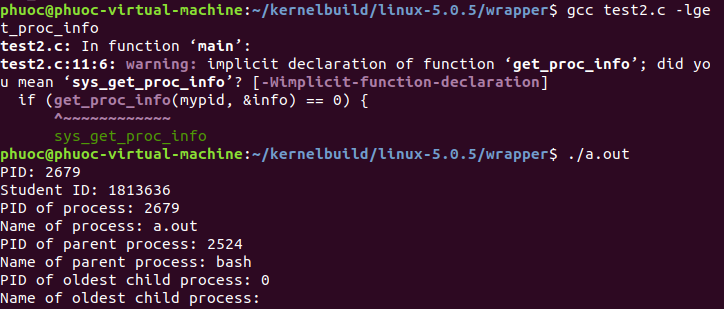
\includegraphics[width=10cm]{10.png}
\caption{Testing}
\end{center}
\end{figure}
%%%%%%%%%%%%%%%%%%%%%%%%%%%%%%%%%
\newpage
\begin{thebibliography}{80}
\bibitem{bib1}
Linux Documentation "https://linux.die.net".
\bibitem{bib2}
GNU Operating System "https://gnu.org/".
\bibitem{bib3}
Make Linux "https://makelinux.net/".
\bibitem{bib4}
UBUNTU Wiki "https://wiki.ubuntu.com".
\bibitem{bib5}
Stackover flow "https://stackoverflow.com".
\end{thebibliography}
\end{document}

